% !TeX program = xelatex
\documentclass[a4paper,10pt]{article}

% ============================================================================
% កិច្ចតែងការបង្រៀនមុខវិជ្ជាគណិតវិទ្យា ថ្នាក់ទី៨ (ម៉ោងសិក្សា ៥០ នាទី — គ្មាន LCD / ប្រើសន្លឹកកិច្ចការជាគោល)
% មេរៀនទី១៧៖ រូបធរណីមាត្រដែលមានវិមាត្របី | ម៉ោងទី៣ (១៧.១.៣)៖ ផ្ទៃក្រឡាខាងនិងផ្ទៃក្រឡាទាំងអស់នៃកោន (ទំ.២២០–២២២)
% វិធីសាស្ត្រ៖ Sector-to-Parallelogram Slicing + Parameter-Trap Contrast (r vs. d, s vs. h) Worksheet
% ============================================================================
\usepackage[a4paper, left=0.95cm, right=0.95cm, top=0.85cm, bottom=0.92cm, footskip=0.52cm]{geometry}
\usepackage{amsmath}
\usepackage{unicode-math}
\usepackage{fontspec}
\usepackage{longtable, array, multirow, colortbl}
\usepackage[table]{xcolor}
\usepackage{enumitem}
\usepackage{pifont}
\usepackage{fancyhdr}
\usepackage{tikz}
\usetikzlibrary{calc, arrows.meta, angles, quotes, patterns, decorations.markings, babel}

\makeatletter
\let\@expl@@@mark@update@singlecol@structures@@\relax
\makeatother

% -------------------- ការស្វែងរកទីតាំងពុម្ពអក្សរដោយស្វ័យប្រវត្តិ (\NGSFindFonts) --------------------
\providecommand{\NGSFindFonts}{%
  \IfFileExists{C:/Windows/Fonts/cambria.ttc}{%
    \def\NGSSysPath{C:/Windows/Fonts/}%
    \def\NGSUserPath{C:/Users/KIT/AppData/Local/Microsoft/Windows/Fonts/}%
  }{%
    \IfFileExists{./fonts/KhmerOSsiemreap.ttf}{\def\NGSSysPath{./fonts/}\def\NGSUserPath{./fonts/}}{%
    \IfFileExists{../fonts/KhmerOSsiemreap.ttf}{\def\NGSSysPath{../fonts/}\def\NGSUserPath{../fonts/}}{%
    \IfFileExists{../../fonts/KhmerOSsiemreap.ttf}{\def\NGSSysPath{../../fonts/}\def\NGSUserPath{../../fonts/}}{%
    \IfFileExists{../../../fonts/KhmerOSsiemreap.ttf}{\def\NGSSysPath{../../../fonts/}\def\NGSUserPath{../../../fonts/}}{%
    \IfFileExists{../../../../fonts/KhmerOSsiemreap.ttf}{\def\NGSSysPath{../../../../fonts/}\def\NGSUserPath{../../../../fonts/}}{%
    \IfFileExists{../../../../../fonts/KhmerOSsiemreap.ttf}{\def\NGSSysPath{../../../../../fonts/}\def\NGSUserPath{../../../../../fonts/}}{%
    \IfFileExists{../../../../../../fonts/KhmerOSsiemreap.ttf}{\def\NGSSysPath{../../../../../../fonts/}\def\NGSUserPath{../../../../../../fonts/}}{%
      \def\NGSSysPath{../../../../../../../fonts/}\def\NGSUserPath{../../../../../../../fonts/}%
    }}}}}}}%
  }%
}
\NGSFindFonts

\setmathfont[Path={\NGSSysPath}, FontIndex=1, Scale=1.02]{cambria.ttc}
\defaultfontfeatures{Ligatures=TeX}

\setmainfont[
  Path={\NGSUserPath},
  Extension=.ttf,
  Script=Khmer,
  BoldFont={KhmerOSsiemreap},
  BoldFeatures={FakeBold=1.8},
  ItalicFont={KhmerOSsiemreap},
  ItalicFeatures={FakeSlant=0.25},
  BoldItalicFont={KhmerOSsiemreap},
  BoldItalicFeatures={FakeBold=1.8, FakeSlant=0.25}
]{KhmerOSsiemreap}

\newfontfamily\muol[
  Path={\NGSUserPath},
  Extension=.ttf,
  Script=Khmer
]{KhmerOSmuollight}

\newfontfamily\NagaBold[
  Path={\NGSUserPath},
  Extension=.ttf,
  Script=Khmer,
  ItalicFont={AKbalthom Naga Bold},
  ItalicFeatures={FakeSlant=0.22}
]{AKbalthom Naga Bold}

\newfontfamily\Tacteing[
  Path={\NGSUserPath},
  Extension=.TTF
]{TACTENG}

\newfontfamily\CalibriPage[
  Path={\NGSSysPath},
  Extension=.ttf
]{calibri}

\newfontfamily\TimesEn[
  Path={\NGSSysPath},
  Extension=.ttf,
  BoldFont={timesbd},
  ItalicFont={timesi},
  BoldItalicFont={timesbi}
]{times}

\newfontfamily\SymbolCirc[
  Path={\NGSSysPath},
  Extension=.ttf
]{cour}
\newcommand{\wcirc}{{\SymbolCirc\fontsize{10.5pt}{12pt}\selectfont o}}

\XeTeXlinebreaklocale "km"
\XeTeXlinebreakskip = 0pt plus 1pt minus 0.1pt

% -------------------- ពណ៌ និងការតុបតែង --------------------
\definecolor{darkred}{RGB}{180, 0, 0}
\definecolor{red5e}{RGB}{210, 15, 15}
\definecolor{headgray}{gray}{0.86}
\definecolor{stepgray}{gray}{0.91}
\definecolor{boxgray}{gray}{0.93}

\pagestyle{fancy}
\fancyhf{}
\renewcommand{\headrulewidth}{0pt}
\fancyfoot[R]{{\CalibriPage\fontsize{9.5pt}{11pt}\selectfont \thepage}}

\setlength{\parindent}{0pt}
\setlength{\parskip}{0pt}
\setlength{\LTpre}{2pt}
\setlength{\LTpost}{2pt}
\setlength{\tabcolsep}{4.5pt}
\arrayrulewidth=0.45pt

\newcolumntype{L}[1]{>{\raggedright\arraybackslash}p{#1}}
\newcolumntype{C}[1]{>{\centering\arraybackslash}p{#1}}

\newcommand{\en}[1]{{\TimesEn #1}}
\newcommand{\enbf}[1]{{\TimesEn\textbf{#1}}}
\newcommand{\unit}[1]{\,\text{\en{#1}}}
\newcommand{\fiveE}[1]{{\NagaBold\fontsize{9.5pt}{13pt}\selectfont\textcolor{red5e}{#1}}}
\newcommand{\timenote}[1]{\textcolor{darkred}{\textit{#1}}}
\newcommand{\khmflourish}{{\Tacteing\fontsize{17pt}{17pt}\selectfont 3}}
\newcommand{\graybox}[1]{\colorbox{boxgray}{\strut\hspace{2pt}#1\hspace{2pt}}}
\newcommand{\ditem}{\tikz[baseline=-0.5ex]\fill (0,0.42ex) -- (0.42ex,0) -- (0,-0.42ex) -- (-0.42ex,0) -- cycle;\hspace{0.3em}}
\newcommand{\cnum}[1]{{\fontsize{10.5pt}{12pt}\selectfont\ding{\numexpr181+#1\relax}}\hspace{0.2em}}
\newcommand{\cfig}[1]{\par\vspace{4pt}{\centering #1\par}\vspace{4pt}}
\newcommand{\stepheader}[1]{\multicolumn{3}{|c|}{\cellcolor{stepgray}\muol #1} \\* \noalign{\hrule height 0.4pt}}
\newcommand{\tri}[1]{\ensuremath{\triangle #1}}

\newcommand{\rightbox}[4][0.18]{%
  \draw[black, line width=0.75pt]
    ($(#3)!#1!(#2)$) -- ($($(#3)!#1!(#2)$)+($(#3)!#1!(#4)$)-(#3)$) -- ($(#3)!#1!(#4)$);
}

% ============================================================================
% រូបធរណីមាត្រ ស-ខ្មៅ (B&W Print-Safe TikZ Figures for Hour 17.3: Cones)
% ============================================================================

% ១. កំណែកិច្ចការផ្ទះទី១០ខ,គ (ទំ.២២៨) និងរំលឹកថាស/រង្វង់
\newcommand{\figPrereqCone}{%
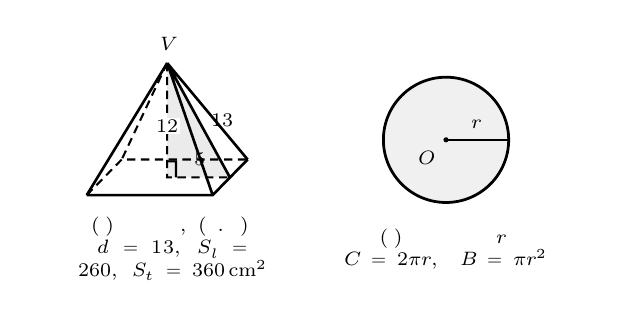
\begin{tikzpicture}[scale=0.78, every node/.style={font=\scriptsize, text=black}]
  % (ក) លំហាត់ទី១០ ខ,គ ទំ.២២៨៖ ពីរ៉ាមីតការេជ្រុង 10, VO=12 => d=13
  \begin{scope}[shift={(-2.20,0)}]
    \coordinate (A) at (-1.40,-0.80);
    \coordinate (B) at (0.65,-0.80);
    \coordinate (C) at (1.22,-0.22);
    \coordinate (D) at (-0.83,-0.22);
    \coordinate (O) at (-0.09,-0.51);
    \coordinate (V) at (-0.09,1.35);
    \coordinate (Z) at (0.93,-0.51);
    \fill[gray!16] (V) -- (O) -- (Z) -- cycle;
    \draw[black, line width=0.95pt] (A) -- (B) -- (C) (V) -- (A) (V) -- (B) (V) -- (C) (V) -- (Z);
    \draw[black, line width=0.75pt, densely dashed] (A) -- (D) -- (C) (V) -- (D) (V) -- (O) -- (Z);
    \rightbox[0.14]{V}{O}{Z}
    \node[above=1pt] at (V) {$V$};
    \node[fill=white, inner sep=0.6pt] at (-0.09,0.32) {$12$};
    \node[above=0.5pt] at (0.45,-0.51) {$5$};
    \node[right=1pt] at ($0.5*(V)+0.5*(Z)$) {$13$};
    \node[align=center, text width=3.45cm] at (0.0,-1.68) {(ក) លំហាត់ទី១០ខ,គ (ទំ.២២៨)៖\\$d=13,\; S_l=260,\; S_t=360\unit{cm}^2$};
  \end{scope}

  % (ខ) រំលឹកបរិមាត្ររង្វង់ និងផ្ទៃថាស
  \begin{scope}[shift={(2.25,0.10)}]
    \draw[black, line width=1.0pt, fill=gray!12] (0,0) circle (1.02cm);
    \fill[black] (0,0) circle (1.2pt) node[below left=0.5pt] {$O$};
    \draw[black, line width=0.9pt] (0,0) -- (1.02,0);
    \node[above=0.5pt] at (0.50,0) {$r$};
    \node[align=center, text width=3.45cm] at (0.0,-1.78) {(ខ) រង្វង់និងថាសកាំ $r$៖\\$C = 2\pi r,\quad B = \pi r^2$};
  \end{scope}
\end{tikzpicture}}

% ២. E1 Engage: មួកក្រដាសរាងកោនបរិវត្ត (កាំ r=2cm, ជនេត្រ s=6cm) ពេលកាត់លាតតាមជនេត្រមួយ
\newcommand{\figEngageCone}{%
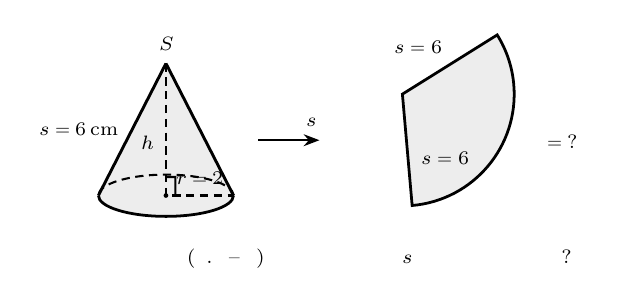
\begin{tikzpicture}[scale=0.78, every node/.style={font=\scriptsize, text=black}]
  % កោន 3D
  \begin{scope}[shift={(-2.55,0)}]
    \coordinate (V) at (0,1.50);
    \coordinate (O) at (0,-0.65);
    \coordinate (R) at (1.10,-0.65);
    \coordinate (L) at (-1.10,-0.65);
    \fill[gray!14] (L) -- (V) -- (R) arc (0:-180:1.10 and 0.34);
    \draw[black, line width=1.0pt] (L) arc (-180:0:1.10 and 0.34);
    \draw[black, line width=0.75pt, densely dashed] (R) arc (0:180:1.10 and 0.34);
    \draw[black, line width=1.05pt] (V) -- (L) (V) -- (R);
    \draw[black, line width=0.8pt, densely dashed] (V) -- (O) -- (R);
    \rightbox[0.14]{V}{O}{R}
    \fill[black] (O) circle (1.1pt);
    \node[above=1pt] at (V) {$S$};
    \node[above=0.5pt] at (0.56,-0.65) {$r=2$};
    \node[left=1.5pt] at ($0.5*(V)+0.5*(L)$) {$s=6\unit{cm}$};
    \node[left=0.5pt] at (0,0.20) {$h$};
  \end{scope}

  \draw[-{Stealth[length=2.0mm]}, line width=0.9pt] (-1.05,0.25) -- (-0.05,0.25) node[midway, above=1pt] {កាត់តាម $s$};

  % ចម្រៀកថាស 2D
  \begin{scope}[shift={(1.95,0.18)}]
    \coordinate (C) at (-0.65,0.82);
    \fill[gray!14] (C) -- ($(C)+(-85:1.82)$) arc (-85:32:1.82) -- cycle;
    \draw[black, line width=1.0pt] (C) -- ($(C)+(-85:1.82)$) arc (-85:32:1.82) -- cycle;
    \node[right=1.5pt] at ($(C)+(-85:1.05)$) {$s=6$};
    \node[above left=0pt] at ($(C)+(32:0.95)$) {$s=6$};
    \node[right=1pt] at ($(C)+(-25:1.85)$) {ធ្នូ $= ?$};
  \end{scope}

  \node[align=center, text width=7.1cm] at (-0.10,-1.68) {មួកក្រដាសរាងកោនបរិវត្ត (ទំ.២២០--២២១)៖ ពេលកាត់ពន្លាតតាមជនេត្រ $s$ តើបានរូបត្រីកោណ ឬចម្រៀកថាស?};
\end{tikzpicture}}

% ៣. E2/E3 ការកាត់ចម្រៀកថាសផ្គុំជាប្រលេឡូក្រាម (ទំ.២២១៖ S_l = pi*r*s) + លំហាត់គំរូទី 2 (កោន+ស៊ីឡាំង)
\newcommand{\figConeSectorComposite}{%
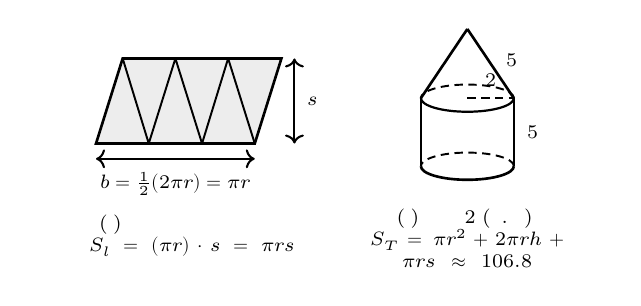
\begin{tikzpicture}[scale=0.72, every node/.style={font=\scriptsize, text=black}]
  % (ក) ចម្រៀកថាស -> ផ្គុំប្រលេឡូក្រាម b = pi*r, កម្ពស់ = s
  \begin{scope}[shift={(-2.25,0.15)}]
    \draw[black, line width=0.95pt, fill=gray!14]
      (-1.85,-0.65) -- (-1.38,0.85) -- (1.42,0.85) -- (0.95,-0.65) -- cycle;
    \draw[black, line width=0.7pt]
      (-0.92,-0.65) -- (-0.45,0.85)
      (0.02,-0.65) -- (0.48,0.85)
      (-1.38,0.85) -- (-0.92,-0.65)
      (-0.45,0.85) -- (0.02,-0.65)
      (0.48,0.85) -- (0.95,-0.65);
    \draw[<->, line width=0.75pt] (-1.85,-0.92) -- (0.95,-0.92) node[midway, below=1pt] {$b = \frac{1}{2}(2\pi r) = \pi r$};
    \draw[<->, line width=0.75pt] (1.65,-0.65) -- (1.65,0.85) node[midway, right=1pt] {$s$};
    \node[align=center, text width=3.95cm] at (-0.15,-2.28) {(ក) ផ្គុំចម្រៀកថាសជាប្រលេឡូក្រាម៖\\$S_l = (\pi r)\cdot s = \pi r s$};
  \end{scope}

  % (ខ) លំហាត់គំរូទី 2 ទំ.២២១៖ សូលីតផ្សំ ស៊ីឡាំង (r=2, h=5) + កោន (s=5)
  \begin{scope}[shift={(2.45,0.10)}]
    \draw[black, line width=0.95pt] (-0.82,-1.00) arc (-180:0:0.82 and 0.24);
    \draw[black, line width=0.7pt, densely dashed] (0.82,-1.00) arc (0:180:0.82 and 0.24);
    \draw[black, line width=0.95pt] (-0.82,-1.00) -- (-0.82,0.20) (0.82,-1.00) -- (0.82,0.20);
    \draw[black, line width=0.8pt] (-0.82,0.20) arc (-180:0:0.82 and 0.24);
    \draw[black, line width=0.7pt, densely dashed] (0.82,0.20) arc (0:180:0.82 and 0.24);
    \coordinate (TopC) at (0,1.42);
    \draw[black, line width=0.95pt] (TopC) -- (-0.82,0.20) (TopC) -- (0.82,0.20);
    \draw[black, line width=0.75pt, densely dashed] (0,0.20) -- (0.82,0.20);
    \node[above=0.5pt] at (0.42,0.20) {$2$};
    \node[right=1.5pt] at (0.82,-0.40) {$5$};
    \node[right=1.5pt] at (0.44,0.86) {$5$};
    \node[align=center, text width=3.45cm] at (0.0,-2.28) {(ខ) គំរូទី \en{2} (ទំ.២២១)៖\\$S_T=\pi r^2+2\pi rh+\pi rs\approx 106.8$};
  \end{scope}
\end{tikzpicture}}

% ៤. E4/E5 ប្រតិបត្តិ ក, ខ (ទំ.២២២) និងលំហាត់ចង្កៀងគោមទី៧ (ទំ.២២៧)
\newcommand{\figElaborateCone}{%
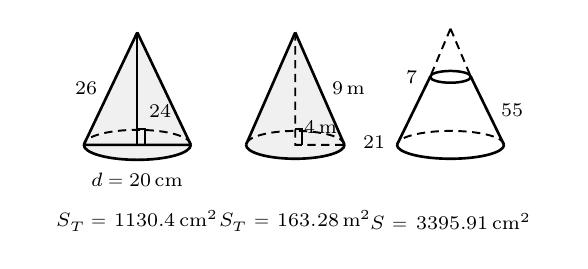
\begin{tikzpicture}[scale=0.68, every node/.style={font=\scriptsize, text=black}]
  % (១) ប្រតិបត្តិ ក (ទំ.២២២)៖ អង្កត់ផ្ចិត d=20cm (r=10), កម្ពស់ h=24cm => s=26cm
  \begin{scope}[shift={(-2.90,0)}]
    \coordinate (V1) at (0,1.35);
    \coordinate (O1) at (0,-0.75);
    \coordinate (L1) at (-1.00,-0.75);
    \coordinate (R1) at (1.00,-0.75);
    \fill[gray!12] (L1) -- (V1) -- (R1) arc (0:-180:1.00 and 0.28);
    \draw[black, line width=0.95pt] (L1) arc (-180:0:1.00 and 0.28) (V1) -- (L1) (V1) -- (R1) (L1) -- (R1);
    \draw[black, line width=0.7pt, densely dashed] (R1) arc (0:180:1.00 and 0.28);
    \draw[black, line width=0.85pt] (V1) -- (O1);
    \rightbox[0.14]{V1}{O1}{R1}
    \node[right=1pt] at (0,-0.12) {$24$};
    \node[below=1pt] at (0,-1.04) {$d=20\unit{cm}$};
    \node[left=1pt] at ($0.5*(V1)+0.5*(L1)$) {$26$};
    \node[align=center, text width=2.55cm] at (0,-2.12) {ប្រតិបត្តិ ក៖\\$S_T=1130.4\unit{cm}^2$};
  \end{scope}

  % (២) ប្រតិបត្តិ ខ (ទំ.២២២)៖ កាំ r=4m, ជនេត្រ s=9m
  \begin{scope}[shift={(0.05,0)}]
    \coordinate (V2) at (0,1.35);
    \coordinate (O2) at (0,-0.75);
    \coordinate (L2) at (-0.92,-0.75);
    \coordinate (R2) at (0.92,-0.75);
    \fill[gray!12] (L2) -- (V2) -- (R2) arc (0:-180:0.92 and 0.26);
    \draw[black, line width=0.95pt] (L2) arc (-180:0:0.92 and 0.26) (V2) -- (L2) (V2) -- (R2);
    \draw[black, line width=0.7pt, densely dashed] (R2) arc (0:180:0.92 and 0.26) (V2) -- (O2) -- (R2);
    \rightbox[0.14]{V2}{O2}{R2}
    \node[above=0.5pt] at (0.48,-0.75) {$4\unit{m}$};
    \node[right=1pt] at ($0.5*(V2)+0.5*(R2)$) {$9\unit{m}$};
    \node[align=center, text width=2.55cm] at (0,-2.12) {ប្រតិបត្តិ ខ៖\\$S_T=163.28\unit{m}^2$};
  \end{scope}

  % (៣) លំហាត់ទី៧ (ទំ.២២៧)៖ ចង្កៀងគោម (កោនធំ r1=21, s1=55 ដកកោនតូច r2=7, s2=10.5)
  \begin{scope}[shift={(2.95,0)}]
    \coordinate (Top) at (0,1.42);
    \draw[black, line width=0.7pt, densely dashed] (Top) -- (-0.38,0.52) (Top) -- (0.38,0.52);
    \draw[black, line width=0.95pt] (-0.38,0.52) -- (-1.00,-0.75) (0.38,0.52) -- (1.00,-0.75);
    \draw[black, line width=0.9pt] (0,0.52) ellipse (0.38 and 0.11);
    \draw[black, line width=0.95pt] (-1.00,-0.75) arc (-180:0:1.00 and 0.26);
    \draw[black, line width=0.7pt, densely dashed] (1.00,-0.75) arc (0:180:1.00 and 0.26);
    \node[left=1pt] at (-0.38,0.52) {$7$};
    \node[left=1pt] at (-0.98,-0.70) {$21$};
    \node[right=1pt] at (0.72,-0.10) {$55$};
    \node[align=center, text width=2.55cm] at (0,-2.12) {ទី៧ ចង្កៀងគោម៖\\$S=3395.91\unit{cm}^2$};
  \end{scope}
\end{tikzpicture}}

% ============================================================================
% ចាប់ផ្ដើមឯកសារ (Document Body)
% ============================================================================
\begin{document}
\fontsize{10pt}{15.2pt}\selectfont

% -------------------- ក្បាលកិច្ចតែងការ (Header) --------------------
\begin{center}
  {\muol\fontsize{11pt}{16pt}\selectfont ព្រះរាជាណាចក្រកម្ពុជា}\\[2pt]
  {\muol\fontsize{10pt}{15pt}\selectfont ជាតិ សាសនា ព្រះមហាក្សត្រ}\\[1pt]
  \khmflourish
\end{center}

\vspace{-26pt}
{\muol\fontsize{9.5pt}{12.8pt}\selectfont
មន្ទីរអប់រំ យុវជន និងកីឡា ខេត្តកំពង់ធំ\\
ការិយាល័យអប់រំ យុវជន និងកីឡា ស្រុកកំពង់ស្វាយ\\
អនុវិទ្យាល័យព្រះក្រសាំង}

\vspace{1pt}
\begin{center}
  {\muol\fontsize{10pt}{14.5pt}\selectfont កិច្ចតែងការបង្រៀន}
\end{center}
\vspace{0pt}

% -------------------- ព័ត៌មានទូទៅ (Metadata) --------------------
{\renewcommand{\arraystretch}{0.98}
\hspace*{4.05cm}%
\begin{tabular}{@{}l l l@{}}
  - \hspace{0.35cm} មុខវិជ្ជា & : & គណិតវិទ្យា ថ្នាក់ទី៨ \\
  - \hspace{0.35cm} ចំណងជើងមេរៀន & : & មេរៀនទី១៧ រូបធរណីមាត្រដែលមានវិមាត្របី \\
  - \hspace{0.35cm} ចំណងជើងរង & : & ១៧.១ ផ្ទៃក្រឡាខាងនិងផ្ទៃក្រឡាទាំងអស់នៃកោន (ទំព័រ ២២០--២២២) \\
  - \hspace{0.35cm} រយៈពេល & : & ១ ម៉ោងសិក្សា (៥០ នាទី) \\
  - \hspace{0.35cm} បង្រៀនដោយ & : & ហុក ប៊ុនថែន \\
  - \hspace{0.35cm} កាលបរិច្ឆេទ & : & ថ្ងៃ\makebox[18mm]{\dotfill}\ ទី\makebox[8mm]{\dotfill}\ ខែ\makebox[18mm]{\dotfill}\ ឆ្នាំ២០២៦ \\
\end{tabular}

\vspace{2pt}

% -------------------- I. វត្ថុបំណង --------------------
\textbf{I.} {\muol វត្ថុបំណង}\\[1pt]
\hspace*{0.55cm}%
\begin{tabular}{@{}l l L{14.2cm}@{}}
  \wcirc \hspace{0.25cm} វិជ្ជាសម្បទា & : & សិស្សប្រាប់បានត្រឹមត្រូវពីធាតុនៃកោនបរិវត្ត (ថាសបាតកាំ $r$ កំពូល កម្ពស់ $h$ និងជនេត្រ $s$) ការពន្លាតផ្ទៃខាងកោនជាចម្រៀកថាស និងរូបមន្តផ្ទៃក្រឡាខាង ($S_l = \pi r s$) ព្រមទាំងផ្ទៃក្រឡាទាំងអស់ ($S_T = \pi r s + \pi r^2 = \pi r(s+r)$) ។ \\
  \wcirc \hspace{0.25cm} បំណិនសម្បទា & : & សិស្សគណនាជនេត្រកោនតាមទ្រឹស្ដីបទពីតាករ ($s = \sqrt{h^2 + r^2}$) និងគណនាផ្ទៃក្រឡាខាង ផ្ទៃក្រឡាទាំងអស់នៃកោន ព្រមទាំងសូលីតផ្សំ (កោន+ស៊ីឡាំង និងចង្កៀងគោម) លើសន្លឹកកិច្ចការបានត្រឹមត្រូវ ។ \\
  \wcirc \hspace{0.25cm} ចរិយាសម្បទា & : & សិស្សមានទម្លាប់ពិនិត្យទិន្នន័យលើរូបកោនដោយប្រុងប្រយ័ត្ន (បែងចែករវាងអង្កត់ផ្ចិត $d$ និងកាំ $r$ ព្រមទាំងកម្ពស់ $h$ និងជនេត្រ $s$) និងឃើញតម្លៃអនុវត្តក្នុងសម្ភារៈប្រើប្រាស់ប្រចាំថ្ងៃ ។ \\
\end{tabular}

\vspace{2pt}

% -------------------- II. សម្ភារៈឧបទេស --------------------
\textbf{II.} {\muol សម្ភារៈឧបទេស}\\[1pt]
\hspace*{0.55cm}$\bullet$ \hspace{0.35cm} សៀវភៅសិក្សាគោលគណិតវិទ្យាថ្នាក់ទី៨ (ទំ.២២០--២២២, ២២៧ និង ២២៩) សន្លឹកកិច្ចការសិស្ស ស-ខ្មៅ (\en{Worksheet\_CONE\_SA} ចំនួន ២ ទំព័រ គ្មាន \en{LCD}) ក្ដារខៀន ដីស បន្ទាត់ក្រិត និងដែកឈាន ។

\vspace{2pt}

% -------------------- III. វិធីសាស្រ្តបង្រៀន --------------------
\textbf{III.} {\muol វិធីសាស្រ្តបង្រៀន}\\[1pt]
\hspace*{0.45cm}%
\begin{tabular}{@{}l l L{14.85cm}@{}}
  $\bullet$ \hspace{0.25cm} គោលវិធី & : & សិស្សមជ្ឈមណ្ឌល (សិក្សាតាមរយៈការបំពេញលើសន្លឹកកិច្ចការជាគោល គ្មាន \en{LCD} និងគ្មានការកាត់បិទក្រដាស) \\
  $\bullet$ \hspace{0.25cm} យុទ្ធវិធីបង្រៀន & : & ស្ថាបនានិយម គម្រូ \en{5Es} រួមបញ្ចូលការផ្គុំចម្រៀកថាសជាប្រលេឡូក្រាម (\en{Sector-to-Parallelogram Mapping}) និងលំហាត់ប្រៀបធៀបអន្ទាក់ទិន្នន័យ (\en{Parameter-Trap Contrast}: $d$ ទល់នឹង $r$, $h$ ទល់នឹង $s$) ។ \\
\end{tabular}
}

\vspace{2pt}

% -------------------- IV. ដំណើរការបង្រៀន --------------------
\textbf{IV.} {\muol ដំណើរការបង្រៀន}

\vspace{1pt}

\renewcommand{\arraystretch}{1.15}
\begin{longtable}{|L{5.50cm}|L{7.90cm}|L{4.80cm}|}
\hline
\rowcolor{headgray}
\multicolumn{1}{|c|}{\muol សកម្មភាពគ្រូ} &
\multicolumn{1}{c|}{\muol ខ្លឹមសារមេរៀន} &
\multicolumn{1}{c|}{\muol សកម្មភាពសិស្ស} \\
\hline
\endfirsthead

\hline
\rowcolor{headgray}
\multicolumn{1}{|c|}{\muol សកម្មភាពគ្រូ} &
\multicolumn{1}{c|}{\muol ខ្លឹមសារមេរៀន} &
\multicolumn{1}{c|}{\muol សកម្មភាពសិស្ស} \\
\hline
\endhead

\hline
\endfoot

\hline
\endlastfoot

% ==================== ជំហានទី១ (2 min) ====================
\stepheader{ជំហានទី១ (រដ្ឋបាលថ្នាក់)}
$\bullet$ ពិនិត្យវត្តមាន សណ្ដាប់ធ្នាប់ អនាម័យ និងចែកសន្លឹកកិច្ចការ \en{Worksheet\_CONE\_SA} ដល់សិស្សគ្រប់គូ \timenote{(2 min)}
&
$\bullet$ រដ្ឋបាលថ្នាក់ និងការត្រៀមសៀវភៅគោល បន្ទាត់ក្រិត ដែកឈាន និងសន្លឹកកិច្ចការសិស្ស
&
$\circ$ ប្រធានថ្នាក់រាយការណ៍វត្តមាន\par\vspace{2pt}
$\circ$ ទទួលសន្លឹកកិច្ចការ និងត្រៀមឧបករណ៍ \\[3pt]
\hline

% ==================== ជំហានទី២ (9 min: ≤3 + 3 + E1 3) ====================
\stepheader{ជំហានទី២ (កិច្ចការផ្ទះ + រំលឹកមេរៀនចាស់ + ទំនាក់ទំនងមេរៀនថ្មី)}
\timenote{(កំណែកិច្ចការផ្ទះ $\le 3\text{ min}$)}\par\vspace{1pt}
$\bullet$ ពិនិត្យចម្លើយលំហាត់ទី៤គ (ទំ.២២៧) និងទី១០ខ,គ (ទំ.២២៨) លើក្ដារខៀនយ៉ាងរហ័ស
&
\textbf{កំណែកិច្ចការផ្ទះ (ទំ.២២៧--២២៨ លំហាត់ទី៤គ និងទី១០ខ,គ)៖}\par\vspace{1pt}
$1.$ \textbf{ទី៤គ៖} $S_{\text{សរុប}} = S_{l,\text{ពីរ៉ាមីត}} + 5\times 10^2 = 240 + 500 = \mathbf{740}$ ឯកតាផ្ទៃ ។\par\vspace{1pt}
$2.$ \textbf{ទី១០ខ,គ៖} អាប៉ូតែម $VZ = \sqrt{12^2+5^2} = 13\unit{cm} \Rightarrow S_l = \frac{1}{2}(40)(13) = \mathbf{260\unit{cm}^2}$;\; $S_t = 260 + 10^2 = \graybox{$360\unit{cm}^2$}$ ។
&
$\circ$ ផ្ទៀងផ្ទាត់និងកែកំណែលំហាត់ទី៤គ និងទី១០ខ,គ ក្នុងសៀវភៅ \\[3pt]

\timenote{(រំលឹកមេរៀនចាស់ 3 min)}\par\vspace{1pt}
$\bullet$ សួរ៖ «ចំពោះរង្វង់និងថាសកាំ $r$ តើបរិមាត្ររង្វង់ $C$ និងផ្ទៃក្រឡាថាស $B$ គណនាតាមរូបមន្តអ្វី? ចុះបើប្រាប់អង្កត់ផ្ចិត $d$ តើកាំ $r$ ស្មើអ្វី?»
&
\textbf{រំលឹករង្វង់ និងថាសកាំ $r$ ($\pi \approx 3.14$)៖}\par\vspace{1pt}
\ditem បើប្រាប់អង្កត់ផ្ចិត $d \Rightarrow$ កាំ $r = \dfrac{d}{2}$ ។\par\vspace{1pt}
\ditem បរិមាត្ររង្វង់៖ $C = 2\pi r$;\quad ផ្ទៃក្រឡាថាស៖ $B = \pi r^2$ ។
&
$\circ$ ឆ្លើយរំលឹករូបមន្ត $r = d/2$, $C = 2\pi r$ និង $B = \pi r^2$ \\[3pt]

& \cfig{\figPrereqCone} & \\[3pt]

\fiveE{E1 - Engage} \timenote{(3 min)}\par\vspace{1.5pt}
$\bullet$ បង្ហាញបញ្ហាមួកក្រដាសលើ \textbf{បេសកកម្មទី១ (\en{E1})} នៃសន្លឹកកិច្ចការ៖\par\vspace{1pt}
\hspace*{0.3em}-- «សិស្សម្នាក់ធ្វើមួកក្រដាសរាងកោនបរិវត្តមានកាំបាត $r=2\unit{cm}$ និងជនេត្រ $s=6\unit{cm}$ ។ ពេលកាត់ពន្លាតផ្ទៃខាងតាមជនេត្រមួយ មិត្ត ក ថាបានរូបត្រីកោណមានបាត $4\unit{cm}$ ឯមិត្ត ខ ថាបានរូបចម្រៀកថាសដែលមានធ្នូស្មើបរិមាត្ររង្វង់បាត $2\pi r$! តើមិត្តណាត្រឹមត្រូវ?»
&
\textbf{១៧.១ ផ្ទៃក្រឡាខាង និងផ្ទៃក្រឡាទាំងអស់នៃកោន}\par\vspace{1.5pt}
\ditem \textbf{បញ្ហាបំផុសគំនិត (\en{E1})៖} ការពន្លាតផ្ទៃកោងនៃកោនតាមជនេត្រ $s$ បង្កើតបាន \textbf{ចម្រៀកថាស} (កាំស្មើជនេត្រ $s$ និងប្រវែងធ្នូស្មើបរិមាត្របាត $2\pi r$) ។
&
$\circ$ អានបេសកកម្មទី១ ពិនិត្យរូបមួកកោន និងគូសធីកទស្សន៍ទាយជាដៃគូ \\[3pt]

& \cfig{\figEngageCone} & \\[3pt]
\hline

% ==================== ជំហានទី៣ (17 min: E2 11 + E3 6) ====================
\stepheader{ជំហានទី៣ (ខ្លឹមសារមេរៀនថ្មី)}
\fiveE{E2 - Explore} \timenote{(11 min: 5 min)}\par\vspace{1pt}
$\bullet$ ឱ្យសិស្សធ្វើជាដៃគូលើ \textbf{ផ្នែកទី១ (ក) ទាញរករូបមន្តផ្ទៃក្រឡាខាងកោនពីចម្រៀកថាស} តាមសៀវភៅទំ.២២០--២២១
&
\textbf{សកម្មភាពរុករកទី១ (ធាតុនៃកោន និងការផ្គុំប្រលេឡូក្រាម)៖}\par\vspace{1pt}
$1.$ \textbf{កោនបរិវត្ត៖} មានបាតជា \textbf{ថាស} កាំ $r$ កម្ពស់ $h$ កាត់តាមផ្ចិតថាសបាត និង \textbf{ជនេត្រ} $s$ មានរង្វាស់ស្មើគ្នាជុំវិញ ($s = \sqrt{h^2 + r^2}$) ។
&
$\circ$ ប្រៀបធៀបពីរ៉ាមីត និងកោនបរិវត្តលើសន្លឹកកិច្ចការ \\[3pt]

$\bullet$ ដើរសួរ៖ «ពេលកាត់ចម្រៀកថាសជាចម្រៀកតូចៗផ្គុំជារាងប្រលេឡូក្រាម តើបាត $b$ និងកម្ពស់នៃប្រលេឡូក្រាមស្មើនឹងអ្វី?»
&
$2.$ បាតប្រលេឡូក្រាមស្មើពាក់កណ្ដាលបរិមាត្របាតកោន៖ $b = \frac{1}{2}(2\pi r) = \pi r$ ហើយកម្ពស់ស្មើជនេត្រ $s \Rightarrow$ ផ្ទៃក្រឡាខាងកោន៖ \graybox{$S_l = \pi r s$} ។
&
$\circ$ បំពេញប្រវែងបាត $\pi r$, កម្ពស់ $s$ និងទាញបាន $S_l = \pi r s$ \\[3pt]

\timenote{(E2 ទី២៖ លំហាត់គំរូទី \en{1} និងទី \en{2} ទំ.២២១ — 6 min)}\par\vspace{1.5pt}
$\bullet$ ដឹកនាំសិស្សបំពេញ \textbf{ផ្នែកទី១ (ខ) គំរូទី \en{1}} (ទំ.២២១៖ $r=2\unit{cm}, s=6\unit{cm}, \pi \approx 3.14$)
&
\textbf{សកម្មភាពរុករកទី២ — លំហាត់គំរូទី \en{1} (ទំ.២២១)៖}\par\vspace{1.5pt}
$\bullet$ ផ្ទៃខាង៖ $S_l = \pi r s \approx 3.14\times 2\times 6 = \mathbf{37.68\unit{cm}^2}$;\; ផ្ទៃបាត៖ $B = 3.14(2^2) = \mathbf{12.56\unit{cm}^2}$ ។\par\vspace{1pt}
$\bullet$ ផ្ទៃក្រឡាទាំងអស់៖ $S_T = S_l + B = 37.68 + 12.56 = \graybox{$50.24\unit{cm}^2$}$ ។
&
$\circ$ គណនាគំរូទី \en{1} បាន $S_l=37.68\unit{cm}^2$, $B=12.56\unit{cm}^2$ និង $S_T=50.24\unit{cm}^2$ \\[3pt]

$\bullet$ ដឹកនាំសិស្សញែកផ្នែកខាងក្រៅទាំង ៣ នៃ \textbf{គំរូទី \en{2}} (ស៊ីឡាំង $r=2, h=5$ + កោន $s=5$)
&
\textbf{លំហាត់គំរូទី \en{2} (ទំ.២២១ — សូលីតផ្សំ ស៊ីឡាំង + កោន)៖}\par\vspace{1.5pt}
$\bullet$ ចែកជា ៣ ផ្នែកខាងក្រៅ (ថាសកណ្ដាលមិនរាប់!)៖\par\vspace{1pt}
\hspace*{0.2em}$S_T = \pi r^2 + 2\pi rh + \pi rs \approx 12.56 + 62.80 + 31.40 = 106.76 \approx \graybox{$106.8$}$ ។
&
$\circ$ ញែកផ្នែកទាំង ៣ នៃគំរូទី \en{2} រកឃើញ $S_T \approx 106.8$ \\[3pt]

& \cfig{\figConeSectorComposite} & \\[3pt]

\fiveE{E3 - Explain} \timenote{(6 min)}\par\vspace{1.5pt}
$\bullet$ ហៅតំណាងគូបង្ហាញ រួចគ្រូសង្ខេបរូបមន្តផ្ទៃក្រឡាកោន (ប្រអប់ទំ.២២១) ឱ្យសិស្សបំពេញ \textbf{ផ្នែកទី២}
&
\textbf{រូបមន្តផ្ទៃក្រឡាខាង និងផ្ទៃក្រឡាទាំងអស់នៃកោន (ទំ.២២១)៖}\par\vspace{1.5pt}
$\bullet$ កោនបរិវត្តមានកាំបាត $r$ និងជនេត្រ $s$៖\par\vspace{1.5pt}
\hspace*{0.3em}$1.$ ផ្ទៃក្រឡាខាង៖ \graybox{$S_l = \pi r s$}\par\vspace{1.5pt}
\hspace*{0.3em}$2.$ ផ្ទៃក្រឡាទាំងអស់៖ \graybox{$S_T = S_l + B = \pi r s + \pi r^2 = \pi r(s + r)$}
&
$\circ$ តំណាងគូឡើងបកស្រាយ\par\vspace{2pt}
$\circ$ បំពេញប្រអប់រូបមន្ត $S_l$ និង $S_T$ ក្នុងផ្នែកទី២ \\[3pt]

$\bullet$ សង្កត់ធ្ងន់លើអន្ទាក់ទិន្នន័យទាំង ២ និងធនាគារហេតុផល \cnum{1}--\cnum{4}
&
\textbf{ចំណុចប្រុងប្រយ័ត្ន និងធនាគារហេតុផល៖}\par\vspace{1.5pt}
$\bullet$ \cnum{1} បើប្រាប់អង្កត់ផ្ចិត $d \Rightarrow r = \frac{d}{2}$ \;\textbar\; \cnum{2} បើប្រាប់កម្ពស់ $h \Rightarrow s = \sqrt{h^2 + r^2}$ \;\textbar\; \cnum{3} $S_l = \pi r s,\; S_T = \pi r(s+r)$ \;\textbar\; \cnum{4} សូលីតផ្សំ/កោនកាត់៖ បូកឬដកតែផ្ទៃខាងក្រៅពិត!
&
$\circ$ កត់ចំណាំអន្ទាក់ $d\to r$ និង $h\to s$ ព្រមទាំងធនាគារហេតុផល \\[3pt]
\hline

% ==================== ជំហានទី៤ (20 min: E4 10 + E5 10) ====================
\stepheader{ជំហានទី៤ (ពង្រីកចំណេះដឹង និងវាយតម្លៃ)}
\fiveE{E4 - Elaborate} \timenote{(10 min: 5 min)}\par\vspace{1pt}
$\bullet$ ឱ្យសិស្សធ្វើជាដៃគូលើ \textbf{ផ្នែកទី៣ (ក) ប្រតិបត្តិ ក (ទំ.២២២, $\pi\approx 3.14$)} ដោយពិនិត្យសញ្ញាកែងត្រង់ផ្ចិតបាត
&
\textbf{៣.ក ប្រតិបត្តិ ក (ទំ.២២២ — ប្រាប់អង្កត់ផ្ចិត $20\unit{cm}$ និងកម្ពស់ $24\unit{cm}$)៖}\par\vspace{1.5pt}
$\bullet$ កាំបាត៖ $r = \frac{20}{2} = \mathbf{10\unit{cm}}$;\; តាមពីតាករ៖ ជនេត្រ $s = \sqrt{24^2 + 10^2} = \sqrt{676} = \mathbf{26\unit{cm}}$ \cnum{1}\cnum{2} ។\par\vspace{1pt}
$\bullet$ ផ្ទៃក្រឡាទាំងអស់៖ $S_T = \pi r(s+r) \approx 3.14\times 10\times (26+10) = 31.4\times 36 = \graybox{$1130.4\unit{cm}^2$}$ ។
&
$\circ$ ចែកអង្កត់ផ្ចិតរក $r=10\unit{cm}$ រកជនេត្រ $s=26\unit{cm}$ រួចគណនា $S_T = 1130.4\unit{cm}^2$ \\[3pt]

\timenote{(E4 ទី២៖ ប្រតិបត្តិ ខ ទំ.២២២ — 5 min)}\par\vspace{1.5pt}
$\bullet$ ឱ្យសិស្សប្រៀបធៀបនិងដោះស្រាយ \textbf{ផ្នែកទី៣ (ខ) ប្រតិបត្តិ ខ (ទំ.២២២)} ដែលប្រាប់កាំ $r=4\unit{m}$ និងជនេត្រ $s=9\unit{m}$ ផ្ទាល់
&
\textbf{៣.ខ ប្រតិបត្តិ ខ (ទំ.២២២ — ប្រាប់កាំ $r=4\unit{m}$ និងជនេត្រ $s=9\unit{m}$ ផ្ទាល់)៖}\par\vspace{1.5pt}
$\bullet$ ផ្ទៃក្រឡាខាង៖ $S_l = \pi r s \approx 3.14\times 4\times 9 = \mathbf{113.04\unit{m}^2}$ ។\par\vspace{1pt}
$\bullet$ ផ្ទៃក្រឡាទាំងអស់៖ $S_T = \pi r(s+r) \approx 3.14\times 4\times (9+4) = 12.56\times 13 = \graybox{$163.28\unit{m}^2$}$ ។
&
$\circ$ សម្គាល់ថាស្គាល់ $r, s$ ស្រាប់ រួចគណនាបាន $S_T = 163.28\unit{m}^2$ \\[3pt]

& \cfig{\figElaborateCone} & \\[3pt]

\fiveE{E5 - Evaluate} \timenote{(10 min: 6 min)}\par\vspace{1pt}
$\bullet$ ឱ្យសិស្សធ្វើ \textbf{ផ្នែកទី៤ (ក) លំហាត់ទី៧ ចង្កៀងគោម (ទំ.២២៧, $\pi\approx 3.14$)} ដោយឯករាជ្យលើសន្លឹកកិច្ចការ
&
\textbf{រង្វាយតម្លៃទី១ — លំហាត់ទី៧ ចង្កៀងគោម (ទំ.២២៧)៖}\par\vspace{1.5pt}
$\bullet$ ចង្កៀងគោមចំហមាត់លើ-ក្រោម (គិតតែផ្ទៃខាងកោនធំ ដកផ្ទៃខាងកោនតូច!)៖\par\vspace{1pt}
\hspace*{0.2em}\ditem កោនធំ ($r_1=21\unit{cm}, s_1=55\unit{cm}$)៖ $S_{l1} = 3.14\times 21\times 55 = 3626.70\unit{cm}^2$ ។
&
$\circ$ វិភាគរូបចង្កៀងគោម និងគណនាផ្ទៃខាងកោនធំ $S_{l1}$ \\[3pt]

$\bullet$ ដើរពិនិត្យការដកផ្ទៃខាងកោនតូច $S_{l2}$ ចេញពីផ្ទៃខាងកោនធំ $S_{l1}$
&
\hspace*{0.2em}\ditem កោនតូច ($r_2=7\unit{cm}, s_2=10.5\unit{cm}$)៖ $S_{l2} = 3.14\times 7\times 10.5 = 230.79\unit{cm}^2$ ។\par\vspace{1pt}
\hspace*{0.2em}$\Rightarrow S_{\text{ចង្កៀងគោម}} = S_{l1} - S_{l2} = 3626.70 - 230.79 = \graybox{$3395.91\unit{cm}^2$}$ ។
&
$\circ$ គណនា $S_{l2}$ រួចទាញបាន $S_{l1} - S_{l2} = 3395.91\unit{cm}^2$ \\[3pt]

\timenote{(E5 បិទបេសកកម្ម \en{E1} និង \en{Exit Check} — 4 min)}\par\vspace{1.5pt}
$\bullet$ សួរបិទបេសកកម្មមួកក្រដាស \en{E1} និងឱ្យសិស្សគូសវង់ \textbf{\en{Exit Check} (ផ្នែកទី៤ ខ)} ដើម្បីវាយតម្លៃរហ័ស
&
\textbf{រង្វាយតម្លៃទី២ — បិទ \en{E1} និង \en{Exit Check}៖}\par\vspace{1.5pt}
$\bullet$ \textbf{ចម្លើយ \en{E1}៖} \textbf{មិត្ត ខ ត្រឹមត្រូវ} — ផ្ទៃខាងកោនពន្លាតបានចម្រៀកថាសមានធ្នូ $2\pi r$ និងផ្ទៃក្រឡា $S_l = \pi r s = 37.68\unit{cm}^2$ ។\par\vspace{1pt}
$\bullet$ \textbf{\en{Exit Check}៖} សំណួរទី១ $\to$ \textbf{គ} ($S_T = \pi r(s+r)$); សំណួរទី២ $\to$ \textbf{ខ} ($s = \sqrt{4^2+3^2} = 5\unit{cm}$); សំណួរទី៣ $\to$ \textbf{ក} ($\pi r^2 + 2\pi rh + \pi rs$) ។
&
$\circ$ ផ្ទៀងផ្ទាត់ចម្លើយ \en{E1}\par\vspace{2pt}
$\circ$ គូសវង់ \en{Exit Check} និងលើកម្រាមដៃបង្ហាញ \\[3pt]
\hline

% ==================== ជំហានទី៥ (≤2 min) ====================
\stepheader{ជំហានទី៥ (កិច្ចការផ្ទះ + បណ្ដាំផ្ញើ)}
\timenote{(ចំណាយពេល $\le 2\text{ min}$)}\par\vspace{1.5pt}
$\bullet$ ដាក់កិច្ចការផ្ទះ (ទំ.២២៧ លំហាត់ទី៦ និងទំ.២២៩ លំហាត់ទី១២) និងណែនាំអានមេរៀនមាឌព្រីស
&
\centerline{\muol កិច្ចការផ្ទះ}\par\vspace{2pt}
$1.$ \textbf{លំហាត់ទី៦ (ទំ.២២៧, រូបទី ១)៖} គណនាផ្ទៃក្រឡាខាង និងផ្ទៃក្រឡាសរុបនៃកោនដែលមានកាំបាត $r=9\unit{cm}$ និងកម្ពស់ $h=16\unit{cm}$ ($\pi\approx 3.14$) ។\par\vspace{1.5pt}
$2.$ \textbf{លំហាត់ទី១២ (ទំ.២២៩)៖} គណនាផ្ទៃក្រឡាសរុបនៃកោន បើផ្ទៃក្រឡាបាតមានរង្វាស់ $160\unit{cm}^2$ និងជនេត្រមានរង្វាស់ $12\unit{cm}$ (យក $\pi \approx 3.142$) ។\par\vspace{1.5pt}
$3.$ \textbf{អានមេរៀនបន្ទាប់៖} ១៧.២ ការគណនាមាឌនៃព្រីស (ទំ.២២២--២២៣) ។
&
$\circ$ កត់ត្រាលំហាត់ទី៦, ទី១២ និងអានមេរៀនមាឌព្រីសជាមុន\par\vspace{2pt}
$\circ$ ជម្រាបលាលោកគ្រូ \\[3pt]
\end{longtable}

% -------------------- កាលបរិច្ឆេទ និងហត្ថលេខា --------------------
\vspace{10pt}
\hfill
\begin{minipage}{9.8cm}
  {\centering
    ថ្ងៃ\makebox[16mm]{\dotfill}\ ខែ\makebox[18mm]{\dotfill}\ ឆ្នាំមមី អដ្ឋស័ក ពុទ្ធសករាជ ២៥៧០\\[2pt]
    កំពង់ស្វាយ, ថ្ងៃទី\makebox[10mm]{\dotfill}\ ខែ\makebox[18mm]{\dotfill}\ ឆ្នាំ២០២៦\\[3pt]
    {\muol គ្រូបង្រៀន}\par}
  \vspace{32pt}
  \hfill{\muol ហុក ប៊ុនថែន}\hspace*{1.4cm}
\end{minipage}

\end{document}
